\documentclass[12pt]{article}
\usepackage{xcolor,comment, subfiles, graphicx, caption, longtable, subfig, fancyhdr}
\usepackage{float} 
\usepackage[a4paper,margin=3cm]{geometry}
\usepackage[hidelinks]{hyperref}
\usepackage[parfill]{parskip}
\usepackage{tikz}
\usepackage{multirow}
\usepackage{listings}
\usepackage{mdframed}
\usepackage{color}
\definecolor{lightgray}{rgb}{.9,.9,.9}
\definecolor{darkgray}{rgb}{.4,.4,.4}
\definecolor{purple}{rgb}{0.65, 0.12, 0.82}

\lstdefinelanguage{JavaScript}{
  keywords={typeof, new, true, false, catch, function, return, null, catch, switch, var, if, in, while, do, else, case, break, const},
  keywordstyle=\color{blue}\bfseries,
  ndkeywords={class, export, boolean, throw, implements, import, this},
  ndkeywordstyle=\color{darkgray}\bfseries,
  identifierstyle=\color{black},
  sensitive=false,
  comment=[l]{//},
  morecomment=[s]{/*}{*/},
  commentstyle=\color{purple}\ttfamily,
  stringstyle=\color{red}\ttfamily,
  morestring=[b]',
  morestring=[b]"
}

\lstset{
   language=JavaScript,
   backgroundcolor=\color{lightgray},
   extendedchars=true,
   basicstyle=\footnotesize\ttfamily,
   showstringspaces=false,
   showspaces=false,
   numbers=left,
   numberstyle=\tiny\color{gray},
   numbersep=9pt,
   tabsize=2,
   breaklines=true,
   showtabs=false,
   captionpos=b
}

\graphicspath{{Images/}}

\definecolor{gray}{rgb}{0.5,0.5,0.5}


% SECTION COMMANDS: here we include some useful commands like ToDo definition, formatting and other purposes
\newcommand\todo[1]{\textcolor{red}{#1}}
\newcommand{\sups}[1]{\ensuremath{^{\textrm{#1}}}}
\newcommand{\subs}[1]{\ensuremath{_{\textrm{#1}}}}
\newcommand{\ic}[1]{\textit{#1}}

\newcommand{\image}[4]{
	\begin{figure}[H]
	\centering
	\includegraphics[width=\linewidth, height = {#1}, keepaspectratio]{#2}
	\caption{#3}
	\label{#4}
	\end{figure}
}

%Alligns two images in a row
\newcommand{\twoimages}[5]{
	\captionsetup[subfigure]{labelformat = empty}
	\begin{figure}[H]
		\begin{center}
	        	\subfloat[#3]{
			\includegraphics[height=#1, keepaspectratio]{#2}
	        	}
        		\hspace{25mm}
	        	\subfloat[#5]{
					\includegraphics[height=#1, keepaspectratio]{#4}
				}
		\end{center}
	\end{figure}
}

\pagestyle{fancy}
\fancyhf{}
\rhead{\color{gray}{\normalsize{VenTour - Design Document - 1.0}}}
\lfoot{\textcolor{gray}{\small{Copyright © 2023, Calcaterra Mirko, Lodetti Emma,  Zallemi Nikolina– All rights reserved}}}
\rfoot{\textcolor{gray}{\thepage}}
\addtocontents{toc}{\protect\thispagestyle{fancy}}

\begin{document}
	\pagenumbering{gobble}
	\begin{titlepage}
		\centering
		\vfill
		{
			
\includegraphics[width =\linewidth, height = 4cm, keepaspectratio]{PolitecnicoLogo.png}
			\label{fig:PolitecnicoLogo}
			\large \\[2ex]M.Sc. Geoinformatics Engineering\\
			\large Hypermedia Applications Project\\[9ex]
			
\includegraphics[width =\linewidth, height = 4cm, keepaspectratio]{Images/VentourLogo.png}\\[9ex]

			\huge Documentation\\[3ex]

            \normalsize \textbf{Group name}: Powerpuff Geoinformatics\\[2.5ex]

			\normalsize \textbf{Calcaterra Mirko}: 10562546\\[0.5ex]
			\normalsize mirko.calcaterra@mail.polimi.it\\[1.5ex]
			\normalsize \textbf{Lodetti Emma}: 10619244\\[0.5ex]
			\normalsize emma.lodetti@mail.polimi.it\\[1.5ex]
            \normalsize \textbf{Zallemi Nikolina}: 10852872\\[0.5ex]
			\normalsize nikolina.zallemi@mail.polimi.it\\[1.5ex]
			\normalsize \today\\[1.5ex]
			\normalsize Version 1.0\\[1.5ex]
   \normalsize Link to Repository: \url{https://github.com/Rkomi98/VenTour}
		}

	\end{titlepage}
	%\maketitle

	\newpage
	\pagenumbering{arabic}
 \section{Introduction}\label{venTour-website}
This is the official documentation file of the Hypermedia Web Application project, course followed in Politecnico di Milano during the Academic year 2022/23

This website has been designed for a Venture Capital Company and can be achieved through this \href{https://rkomi98.github.io/VenTour/}{link}. In the \href{https://github.com/Rkomi98/VenTour}{\textbf{repository}} it is possible also to find the Design document and the implementation code (and usability inspection?) of the website.

Now we will see first the requirements, some constraints about the relationships of the main entities of the website. The project is divided into four main parts: Design, Backend, Frontend, and Usability test.

\subsection{Requirements}\label{requirements}
Before starting you have to download or fork the project on your PC and follow the installation of \href{https://nodejs.org/en}{NodeJS}. Once done, you have to run in both Backend and Frontend folders:

\begin{lstlisting}
npm install
\end{lstlisting}

When everything is ready, use in the backend folder to ensure that everything is ok there:

\begin{lstlisting}
node index.js
\end{lstlisting}

Therefore go in the frontend folder and run the project:

\begin{lstlisting}
npm run dev
\end{lstlisting}

\subsection{Architecture}\label{architecture}
In this section, we talk about the high-level structure and organization of the hypermedia application. It describes the major components and their relationships, providing an understanding of how different sections of the system work together to achieve the specific functionality.

\begin{enumerate}
    \item \textbf{System Components}: The repository is split into two main parts: Backend and Frontend. We will better focus on the specific sections, respectively (\ref{sec: Backend}, \ref{sec: Frontend}). In 'Backend' folder, you can find the relational database and the package needed to run the application (see the section \ref{sec: Backend} for more information). The folder 'Frontend' contains everything related to the design and implementation of the website, so all the HTML/CSS codes needed to display all the pages together, and the JavaScript scripts used to run the website. The folder "components" contains all the VUE components used in one or more pages of the website. %, and the function used to see some interactive tool developed on the website
    
    \item \textbf{Component Interaction}: Backend and frontend communicate with each other thanks to JavaScript functions:
    
\begin{lstlisting}
const { data: WhatYouWantToRetrieve } = await useFetch(
    useRuntimeConfig().public.serverURL + '/WhatYouWantToRetrieveFolder'
);
\end{lstlisting}

Remember to run Backend, with and the command in the terminal:

\begin{lstlisting}
node index.js
\end{lstlisting}

And Frontend with the command:

\begin{lstlisting}
npm run dev
\end{lstlisting}

\item \textbf{Data Flow}: All data is static and is stored in the file \texttt{dbInit.js}. It means that it is not updated externally by the user but can be updated only by the developer who can add new fields or modify the ones already existing in the \texttt{dbInit.js} file and the \texttt{index.js} file.
\item \textbf{Scalability and Performance}: The website is optimized for both mobile and desktop. We simplified some features in the mobile version of the code in order to make the application faster and more usable.
\item \textbf{Deployment Considerations}: All the code needed to run the application is contained in this repository, and the host of the website used to run this application online is \href{https://pages.github.com/}{\textbf{GitHub Pages}}.
\item \textbf{Technologies Used}: The website has been developed using the Vue.js framework together with Node.js, and it has been published online using \textbf{GitHub Pages}. The project utilized various technologies, frameworks, and tools.
\item \textbf{Hosting Service}: We decided to use \textbf{GitHub Pages} because we designed a static website and we don't need to update the database when the user needs.
\item \textbf{Rendering Mode}: We don't need to update data frequently and we prefer not to pre-render pages to maintain good performance of the website. Therefore, we excluded the Client-Side Rendering (CSR) method. Since we didn't have dynamic data in our database design, we decided not to use Server-Side Rendering (SSR) either. That's why we used \textbf{Static Site Generation (SSG)} instead. With static site generation, the pages \textit{fetch data once during build-time}. You can see it running the command \texttt{node index.js} in the Backend folder. We chose static-generated pages because they are very fast and perform well since all the pages are built beforehand. We needed to maximize performance on all devices. In general, SSG is perfect for pages, which aligns with our case.\\
Also SSG can give to the website a better \textbf{scalability} (it can be easily cached) and an improved \textbf{security} without executing server-side code.

\end{enumerate}

\section{Design}
Design in-the-large with C-IDM, and in the small with the Wireframes can be found, together with use case scenarios and database design, in the Design Document (see "Design Document" folder in "Documents" in the repository).

\section{Backend}\label{sec: Backend}

Backend is mainly made by 4 files, two JavaScript files and two json files:

    \begin{itemize}
        \item \textbf{dbInit.js}: all data of the database needed in the website is contained and defined here. This file is mainly split in three parts, related to the three main components of the database: Area, Company and People.
        \item \textbf{index.js}: in this file the definition of all tables needed to make the website working is contained. The Server is initialized with area, company and people. Here you can find all the field related to those table. They are connected one each other, as defined in the Relational schema of the database (figure \ref{fig: RS}).
        \begin{figure}[h]
            \centering
\tikzset{every picture/.style={line width=0.75pt}} %set default line width to 0.75pt        

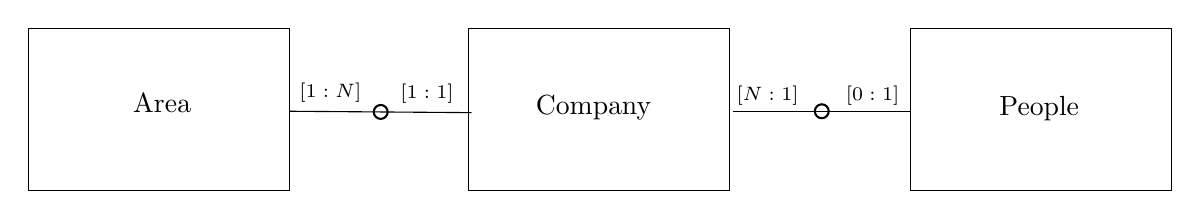
\begin{tikzpicture}[x=0.75pt,y=0.75pt,yscale=-1,xscale=1]
%uncomment if require: \path (0,300); %set diagram left start at 0, and has height of 300

%Shape: Rectangle [id:dp3659909958648019] 
\draw   (56,81) -- (182,81) -- (182,159) -- (56,159) -- cycle ;
%Shape: Rectangle [id:dp2422134142262965] 
\draw   (268,81) -- (394,81) -- (394,159) -- (268,159) -- cycle ;
%Shape: Rectangle [id:dp3572877535613289] 
\draw   (481,81) -- (607,81) -- (607,159) -- (481,159) -- cycle ;
%Straight Lines [id:da9954348081189233] 
\draw    (182,121) -- (269.67,121.67) ;
\draw [shift={(225.83,121.33)}, rotate = 0.44] [color={rgb, 255:red, 0; green, 0; blue, 0 }  ][line width=0.75]      (0, 0) circle [x radius= 3.35, y radius= 3.35]   ;
%Straight Lines [id:da6323853765632855] 
\draw    (395.67,121) -- (481,121) ;
\draw [shift={(438.33,121)}, rotate = 360] [color={rgb, 255:red, 0; green, 0; blue, 0 }  ][line width=0.75]      (0, 0) circle [x radius= 3.35, y radius= 3.35]   ;

% Text Node
\draw (105.33,111) node [anchor=north west][inner sep=0.75pt]   [align=left] {Area};
% Text Node
\draw (299.33,112.33) node [anchor=north west][inner sep=0.75pt]   [align=left] {Company};
% Text Node
\draw (522.67,112.33) node [anchor=north west][inner sep=0.75pt]   [align=left] {People};
% Text Node
\draw (185.33,106.07) node [anchor=north west][inner sep=0.75pt]  [font=\scriptsize]  {$[ 1:N]$};
% Text Node
\draw (234,106.73) node [anchor=north west][inner sep=0.75pt]  [font=\scriptsize]  {$[ 1:1]$};
% Text Node
\draw (396,107.4) node [anchor=north west][inner sep=0.75pt]  [font=\scriptsize]  {$[ N:1]$};
% Text Node
\draw (448.67,107.4) node [anchor=north west][inner sep=0.75pt]  [font=\scriptsize]  {$[ 0:1]$};


\end{tikzpicture}

            \caption{Relational schema of the database}
            \label{fig: RS}
        \end{figure}
        
        \item \textbf{package-lock.json}: here all the package and modules needed are defined, in order to make the website working. 
        \item \textbf{pagkage.json}: General information about the application with the dependencies needed.
    \end{itemize}
    The list of extra modules imported in the project and that you need to install are the following:
\begin{itemize}
    \item \textbf{"cors"}: used to fix the localhost address (link used to open the project):
    \begin{lstlisting}
const corsOptions = { origin: "http://localhost:3000" // The link of your project when run locally }
    \end{lstlisting}
    \item \textbf{"express"}: It is used to manage the routing and the get function in HTTP methods
    \item \textbf{"sequelize"} and \textbf{"sqlite3"}: are used to work in SQL and manage database.
\end{itemize}
\subsection{Server}
In access of the Database you need some parameters, in areas, companies and people you need:
    \begin{itemize}
        \item \textbf{id} (\textit{required}): The ID of the area/person/company the user wants to retrieve from the database.
    \end{itemize}
        The response can be:
        \begin{itemize}
            \item \textbf{200 OK} - Area/Person/Company data returned successfully.
            \item \textbf{404 Not Found} - Object not found.
        \end{itemize}
\section{Frontend}\label{sec: Frontend}
Frontend folder is split in many folders and many files:
\begin{itemize}
    \item In \textbf{assets}, you can find some of the images used in the website (some others are directly retrieved by link from the web) and the global CSS model of the website. Here, in particular, the tailwind library is defined. Additionally, the \texttt{default.vue} file in the layout folder provides a default setting.
    \item In \textbf{components}, there are all the components that have been used in the pages of the website. By components, we mean modular, reusable, and self-contained units of code that perform specific functions. They act as building blocks or pieces of code that encapsulate related functionality and data together.
    \item The \textbf{dist} folder is used only to render the GitHub page online. It is essentially one folder of the \textbf{output} folder, which is used to render the entire website.
    \item The \textbf{pages} folder contains all the pages of the website. The order maintains the structure found in the website, so the branches will be in folders and the leaves in subfolders.
\end{itemize}

In \texttt{package.json}, there is a list of extra modules imported in the project:
\begin{itemize}
    \item \texttt{"autoprefixer"}: A tool that automatically adds vendor prefixes to CSS properties, ensuring better cross-browser compatibility.
    \item \texttt{"gh-pages"}: A utility for publishing web pages directly from a Git repository to GitHub Pages.
    \item \texttt{"nuxt"}: A Vue.js framework for building static websites.
    \item \texttt{"postcss"}: A tool for transforming CSS styles using JavaScript plugins, enabling tasks such as autoprefixing, minification, and more.
    \item \texttt{"tailwindcss"}: A highly customizable CSS framework that provides utility classes for quickly building responsive and modern user interfaces. We used it only for the form in the "Get in Touch" section.
\end{itemize}
\section{Functionalities}
The main components of the application are:
\begin{itemize}
  \item \textbf{Carousel}: Carousel component is used to display a set of images or content in a slideshow format. It allows users to navigate through the images or content horizontally. It is used in the "About us" section to show the most relevant moments in the history of the company. The Carousel is made up of 6 slides, and on the right and left, there are two arrows that allow you to go to the next and previous slide. Each slide contains a header with a paragraph, enclosed in a container with low opacity. A specific image is displayed as the background for each slide.
  
  \begin{figure}[h]
    \centering
    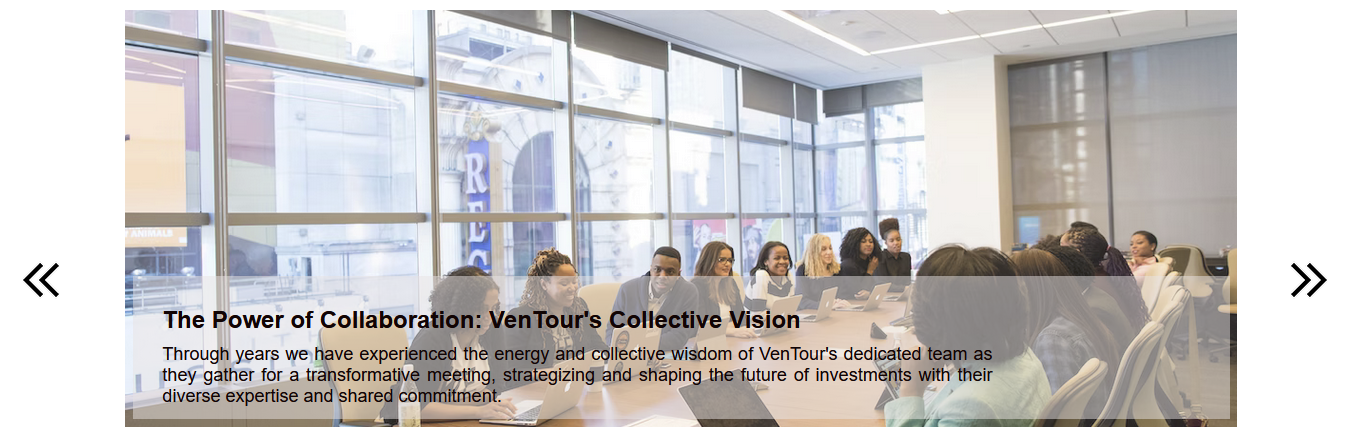
\includegraphics[width=0.6\textwidth]{Images/Carousel.png}
    \caption{Carousel example}
  \end{figure}
  
  \item \textbf{Cards}: Cards are UI components that represent a small, self-contained unit of content. Cards could contain the following information:
    \begin{itemize}
      \item Image, Area, and role of people working in the company in the "Our Team" section.
      \item Logo, CEO, and Area of companies of Investments in the "Investments" section.
    \end{itemize}
    Each card has the following properties:
    \begin{itemize}
      \item \textbf{title}: The main information to display. It is the name of the person in the "Our Team" section and the CEO in the "Investments" section.
      \item \textbf{subtitle}: The second information to display. It is the role and area in the company for people in the "Our Team" section and the area in "Investments".
      \item \textbf{link}: Link to the page description in both "Our Team" and "Investments" sections.
      \item \textbf{img}: Image of the person who works in VenTour and the icon of the company.
    \end{itemize}
  
  \begin{figure}[h]
    \centering
    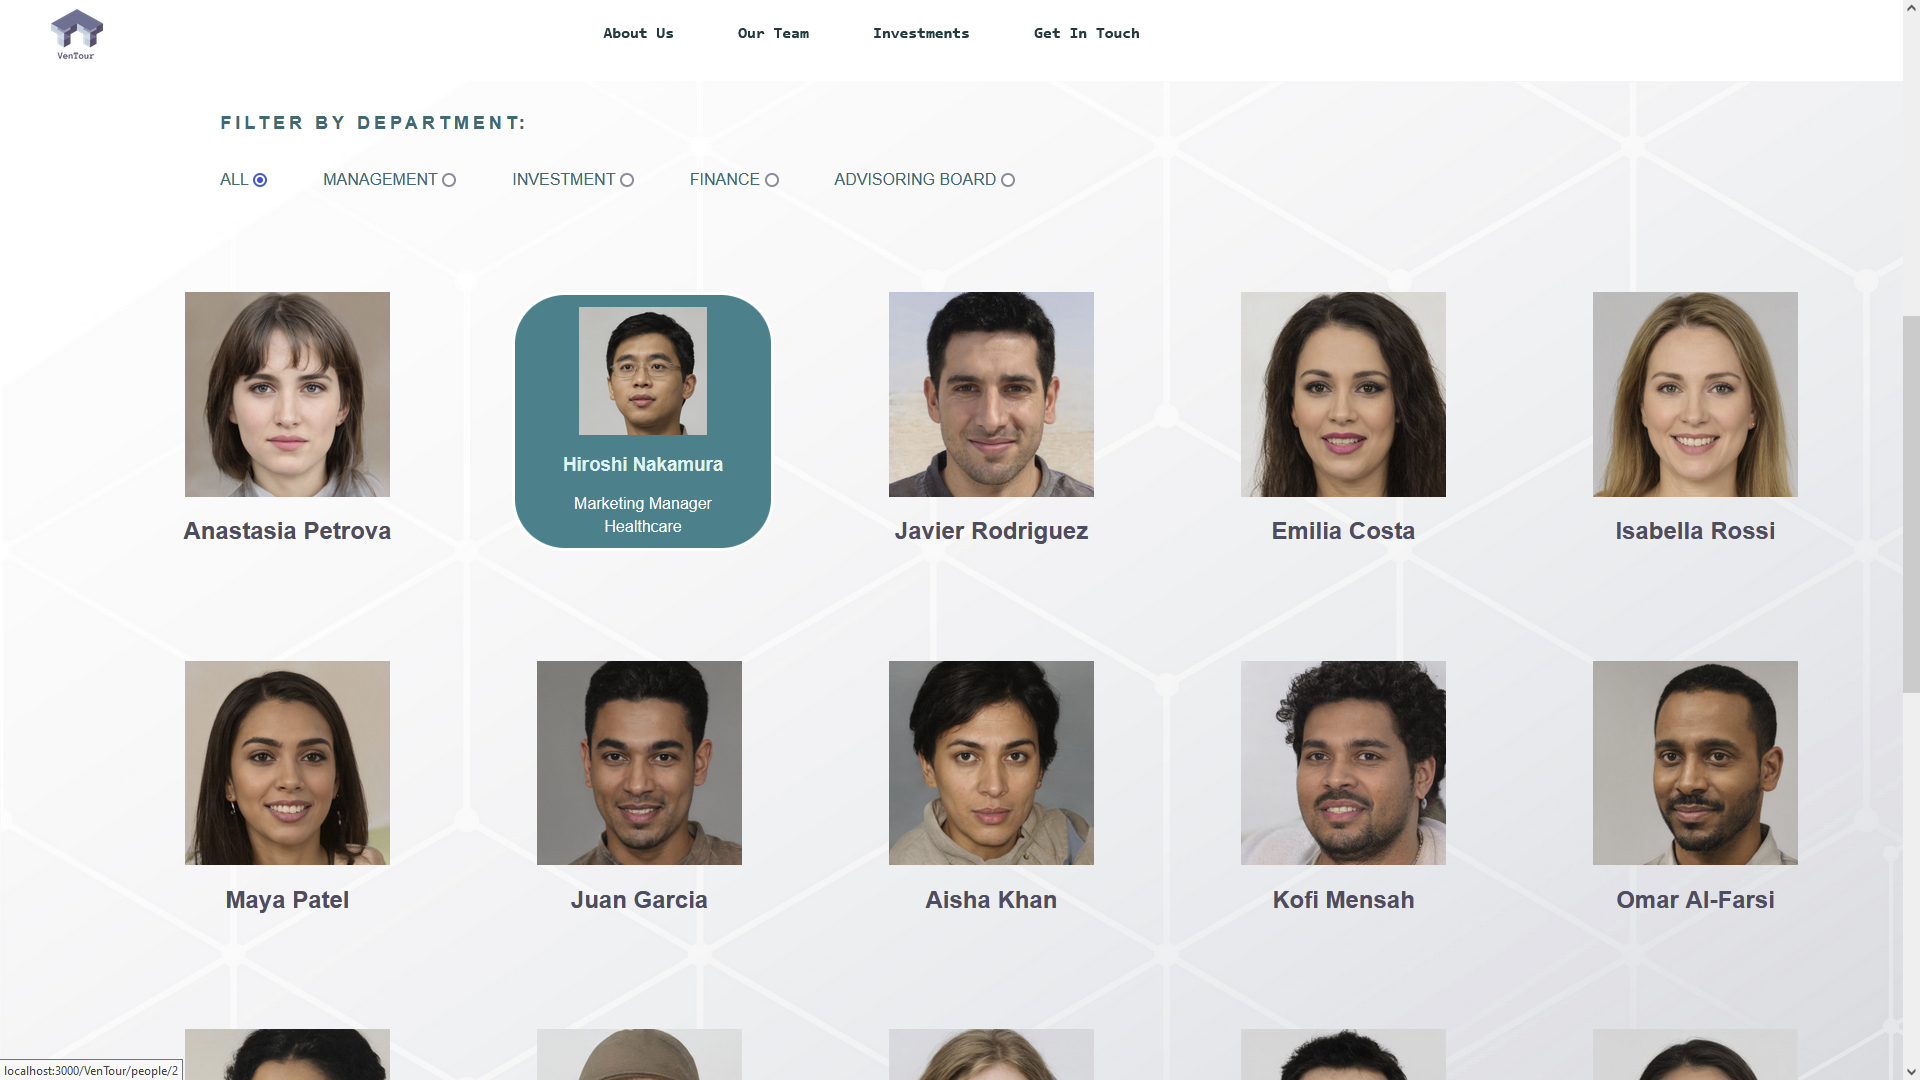
\includegraphics[width=0.6\textwidth]{Images/Cards01.png}
    \caption{Cards example}
  \end{figure}
  
  \item \textbf{Footer}: The footer component appears at the bottom of the webpage or application screen and provides information about:
    \begin{itemize}
      \item Copyright notes
      \item Services and contacts links
      \item Social media links
    \end{itemize}
    The main properties of the footer are:
    \begin{itemize}
      \item \textbf{Service}: External and useful link.
      \item \textbf{Contact}: Main information to keep in contact with VenTour.
      \item \textbf{Social Media icons}: Icons of the three main social media platforms used by VenTour (Facebook, Instagram, and LinkedIn).
    \end{itemize}
  
  \begin{figure}[h]
    \centering
    
\includegraphics[width=0.6\textwidth]{Images/Footer.png}
    \caption{Footer example}
  \end{figure}
  
  \item \textbf{Header}: The header component is located at the top of the webpage. It includes the logo and navigation menus to the main pages of the website (About us, Our team, Investments, and Get in Touch). The header differs between mobile and desktop versions. In the mobile version, a hamburger menu is displayed, allowing the user to choose among the sections by clicking on the three rows. In the desktop version, all sections are visible in the header. Below are examples of both versions:
  
  \begin{figure}[h]
    \centering
    
\includegraphics[width=0.4\textwidth]{Images/Header01.png}
    \caption{Header in mobile version}
  \end{figure}
  
  \begin{figure}[h]
    \centering
    
\includegraphics[width=\textwidth]{Images/Header02.png}
    \caption{Header in desktop version}
  \end{figure}
  
  \item \textbf{Supervisor}: Assigns the right supervisor to each company. It has a single property, which is the name of the supervisor.
  
  \begin{figure}[h]
    \centering
    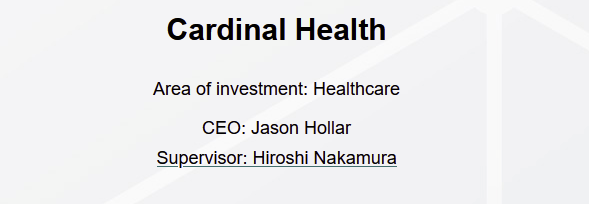
\includegraphics[width=0.4\textwidth]{Images/Supervisor.png}
    \caption{Supervisor example}
  \end{figure}
  
  \item \textbf{CardSection}: Cards in this section are made up of clickable containers. Each container displays the company's image and two subtitles with the name of the CEO and the area. Here is an example:
  
  \begin{figure}[h]
    \centering
    
\includegraphics[width=0.6\textwidth]{Images/CardSection.png}
    \caption{CardSection example}
  \end{figure}
  The properties of the CardSection include:
  \begin{itemize}
    \item Image container with the logo
    \item Two subtitles with the name of the CEO and the area the company mainly addresses.
  \end{itemize}
  \item \textbf{AreaFilter}: It gives to each area card the name and the possibility to filter in the Company/index.vue file (Investment page). It allow also to go in the page of each area. It is made by a logo, the name of the area, data\_target (numbers of companies helped in the story of VenTour in the specific area) and the link to the specific area page.
  \item \textbf{AreaHeader}: it allows to show a dropdown menu with all the area fields that are present in the database. Clicking on this menu in the header, it is possible to go in each specific area page. It is simply made by the name of the area and the link to go in its page.
  \item \textbf{AreaHome}: each area has its card in the home page. Thanks to this component, each field can have its specific box. The main elements are the link to the area page, the name of the area and a small description of the area split in 3 elements, one of the three is highlighted.
  \item \textbf{AreaIdPage}: Small components which show, in each company, the area where it is inserted in. It is made by the name of the area and the link to achieve the specific page.
  \item \textbf{CarouselCompany}: component that is used to 
\end{itemize}

\subsection{Extra functionalities implemented}
The main two extra functionalities we added in the website are:
\begin{itemize}
    \item \textbf{Filters}. There are two different filters, implemented in two different pages:
    \begin{itemize}
        \item \textbf{Our Team}: simple filter that is used only to filter people by team. 
        \item \textbf{Investments}: more complicated filter which is used to filter company by the following paramater:
        \begin{itemize}
            \item \textbf{Most Relevant}: you can select even all of them or only the most relevant
            \item \textbf{Area}: you can select the company by area
            \item \textbf{Search}: You can also search for the company to see if it is in the investments agreement
        \end{itemize}
    \end{itemize}
    \item \textbf{Form} In Get In touch page there are two forms, one is made to send a request to be present in the list of investments of Ventour, the other one is to send an application and so to be part of the Ventour team.
\end{itemize}

\section{SEO optimization}

\section{Work flow}
All the people of the group have worked on all the pages and almost all the files, somebody focusing more on the backend and components creation (Mirko Calcaterra, Emma Lodetti) and Nikolina Zallemi more on the design and the frontend. For more information about the the specific workflow, we suggest you to pay attention to the \href{https://github.com/Rkomi98/VenTour/commits/main}{list of commit} or clicking on each file in the repository and select the "Blame" view.

    
\end{document}
